\documentclass{article}
\usepackage{amsmath}
\usepackage{graphicx}
\usepackage{float}
\usepackage{hyperref}
\usepackage{fancyvrb}
\usepackage{enumitem}
\usepackage{matlab-prettifier}
\setlength{\parindent}{0pt}
\graphicspath{{../images/}}

\title{CS663: Digital Image Processing - Homework 4}
\author{Harsh $\vert$ Pranav $\vert$ Swayam} 
\date{October 22, 2024}

\begin{document}

\maketitle
\section{Homework 4 - Question 4}

\subsection*{For ORL Dataset:}

\begin{figure}[!htb]
    \centering
    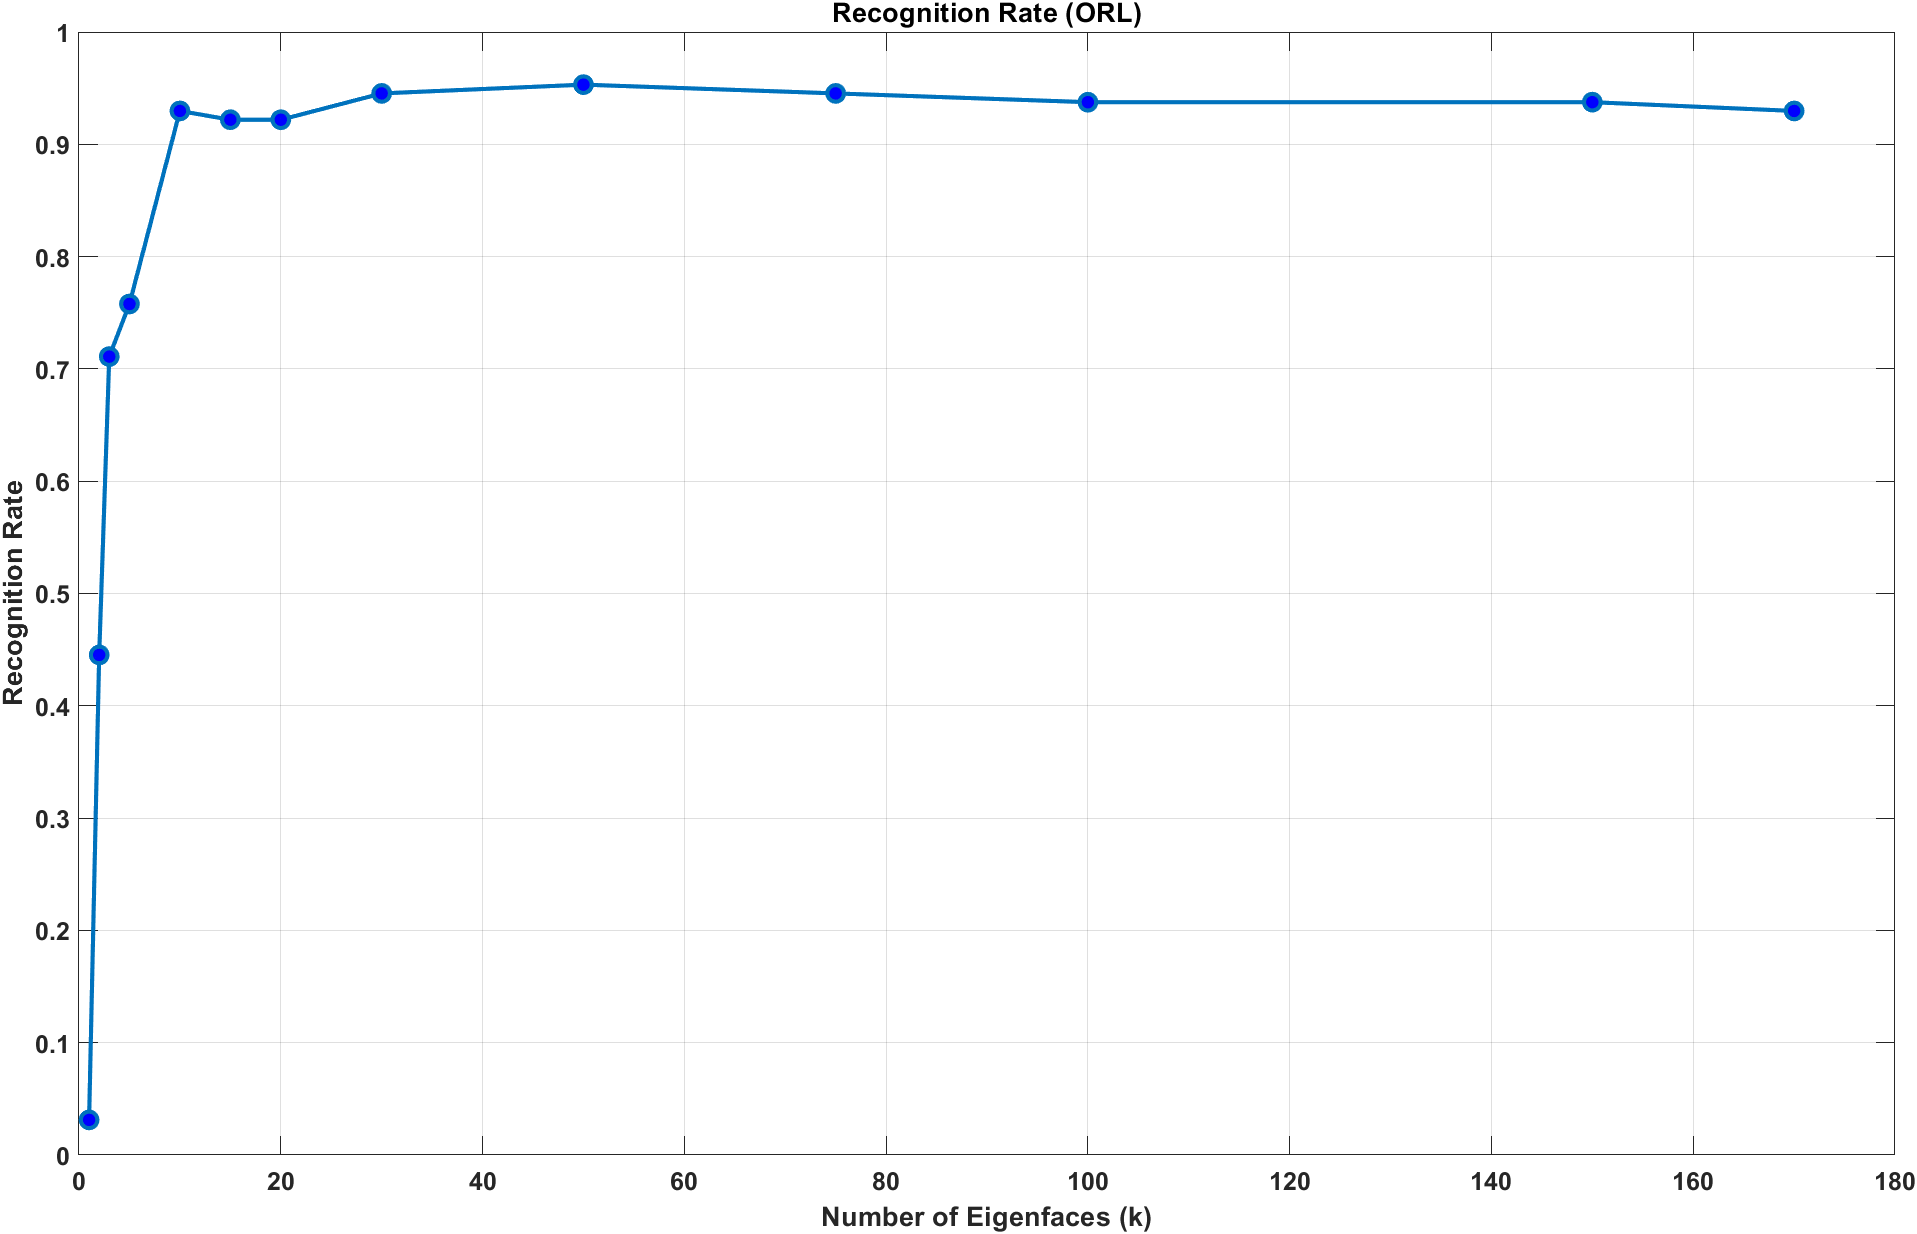
\includegraphics[width=0.6\textwidth]{recog_orl_eig.png}
    \caption{Recognition Rate using the \texttt{eig} method for ORL dataset}
\end{figure}

\begin{figure}[!htb]
    \centering
    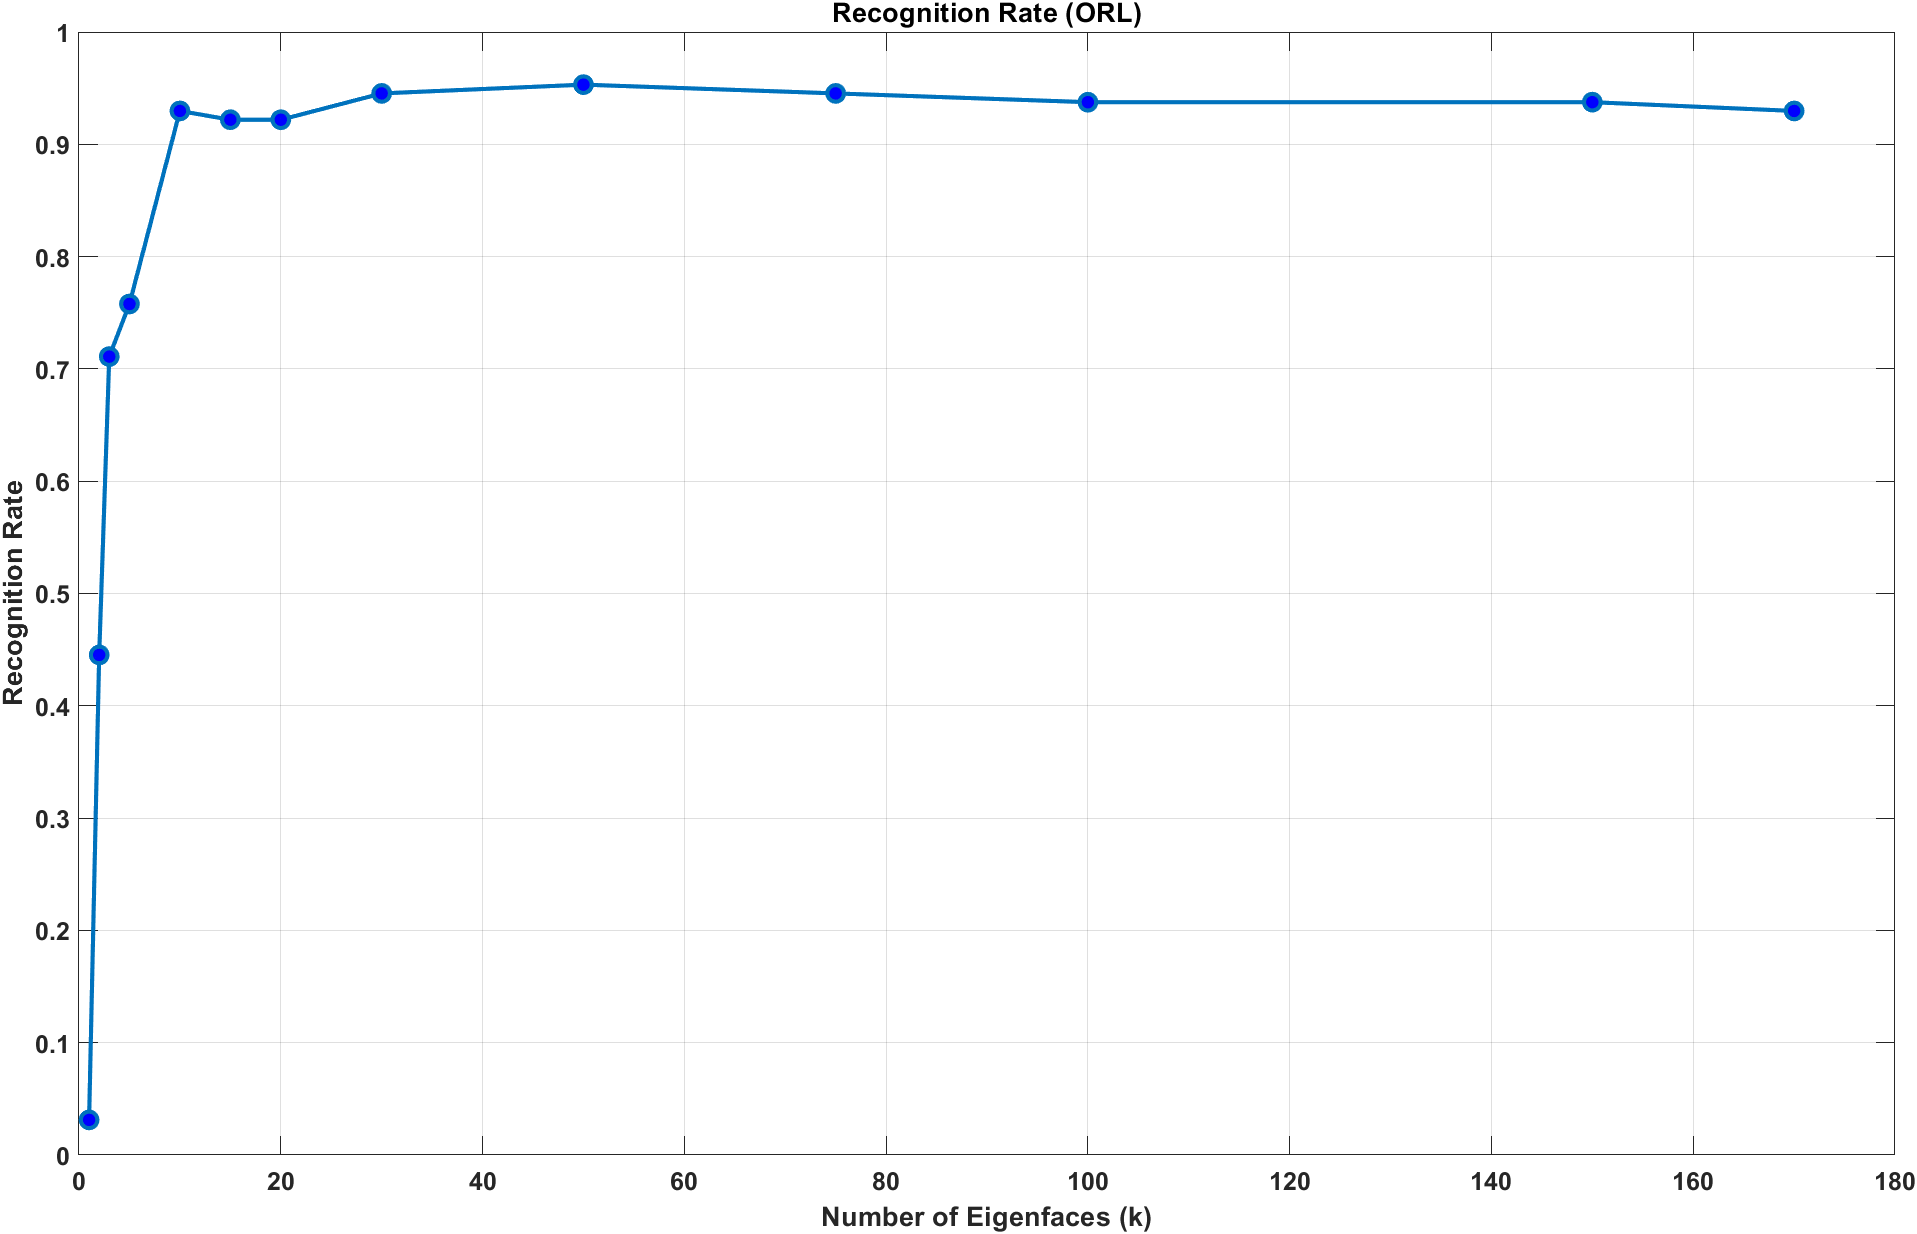
\includegraphics[width=0.6\textwidth]{recog_orl_svd.png}
    \caption{Recognition Rate using the \texttt{svd} method for ORL dataset}
\end{figure}

\newpage
\subsection*{For Yale Dataset:}

\textbf{(a) All eigencoefs:}

\begin{figure}[!htb]
    \centering
    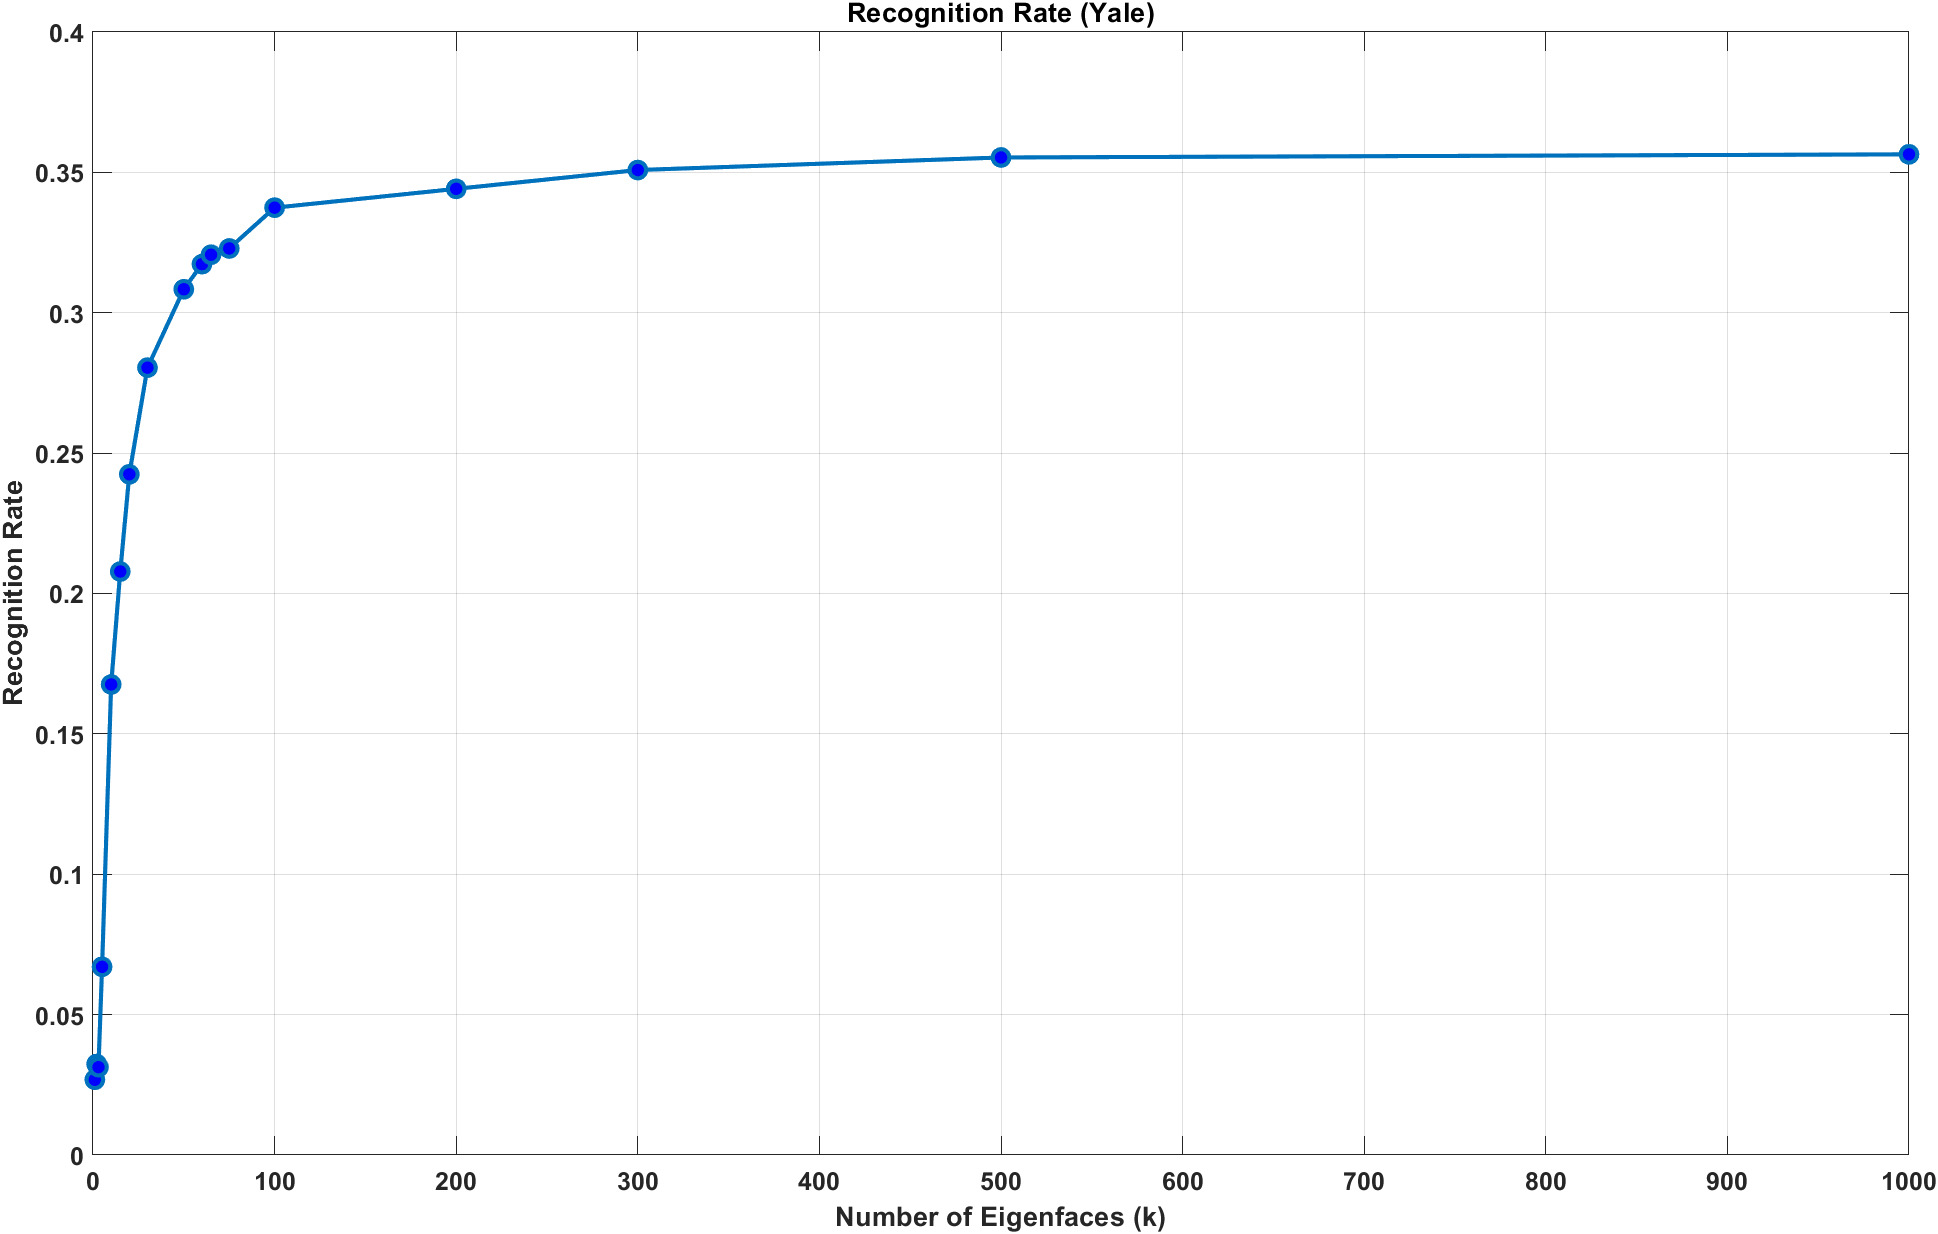
\includegraphics[width=0.6\textwidth]{recog_yale.png}
    \caption{Recognition Rate using all the eigencoefficients for Yale dataset}
\end{figure}

\textbf{(b) Excluding top 3 eigencoefs:}

\begin{figure}[!htb]
    \centering
    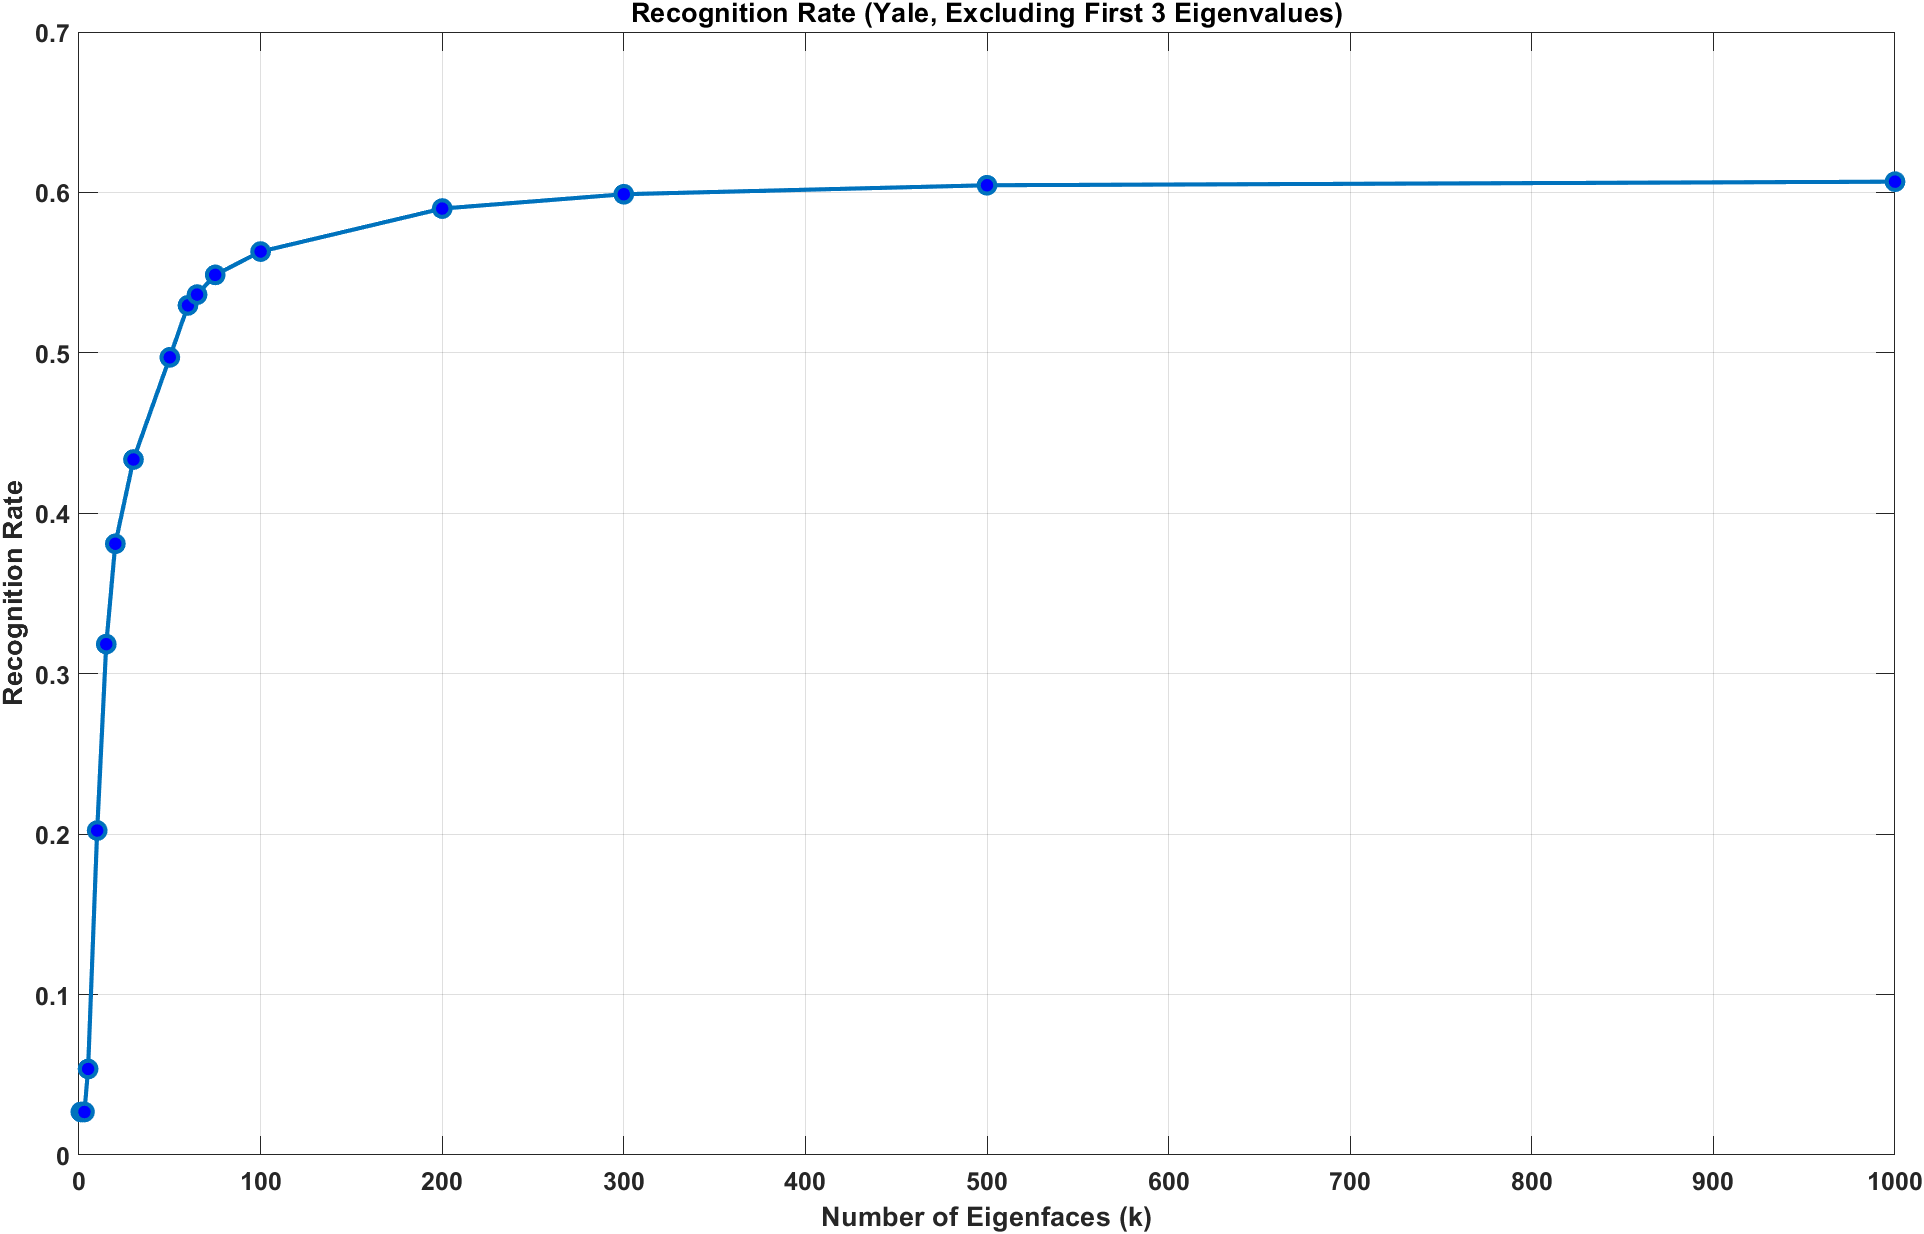
\includegraphics[width=0.6\textwidth]{recog_yale_excluded.png}
    \caption{Recognition Rate using all \textit{except 3} eigencoefficients corresponding to the largest eigenvalues for Yale dataset}
\end{figure}

\textbf{Observation:} It can be seen from both the plots that neglecting the top 3 eigen coefs gives better results since it will lead to more filtering of low light illumination

\newpage
\subsection*{Reconstruction of Image (from ORL):}

The reconstructed images for an example from the ORL dataset are as follows:

\begin{figure}[!htb]
    \centering
    \begin{minipage}[b]{0.3\textwidth}
        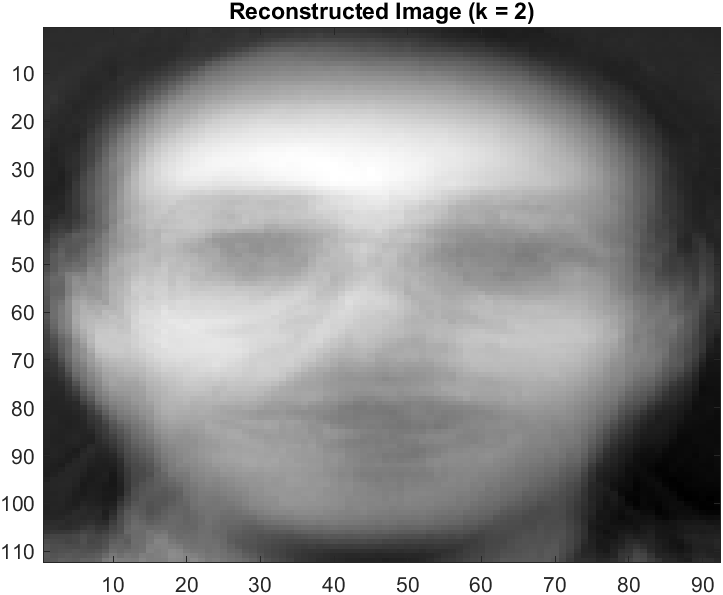
\includegraphics[width=\textwidth]{orl_recon_2.png}
        % \caption{Noisy \texttt{barbara256}}
    \end{minipage}
    % \hfill
    \begin{minipage}[b]{0.3\textwidth}
        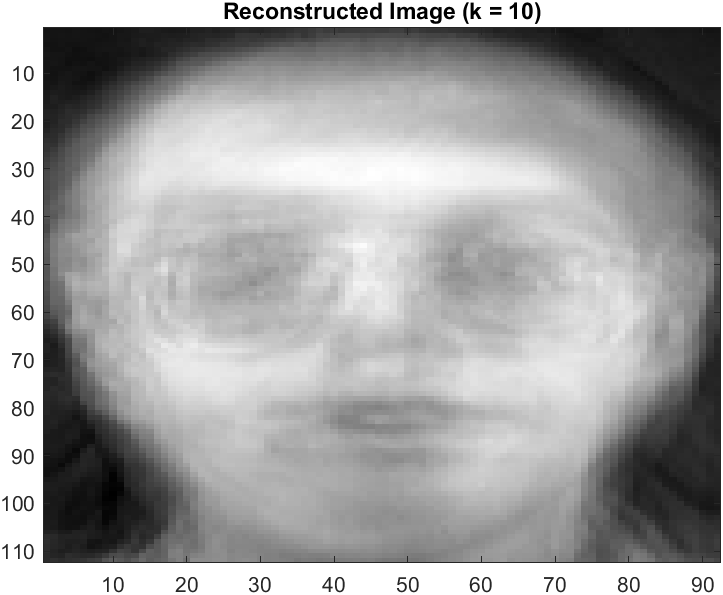
\includegraphics[width=\textwidth]{orl_recon_10.png}
        % \caption{Noisy \texttt{kodak24}}
    \end{minipage}
    % \hfill
    \begin{minipage}[b]{0.3\textwidth}
        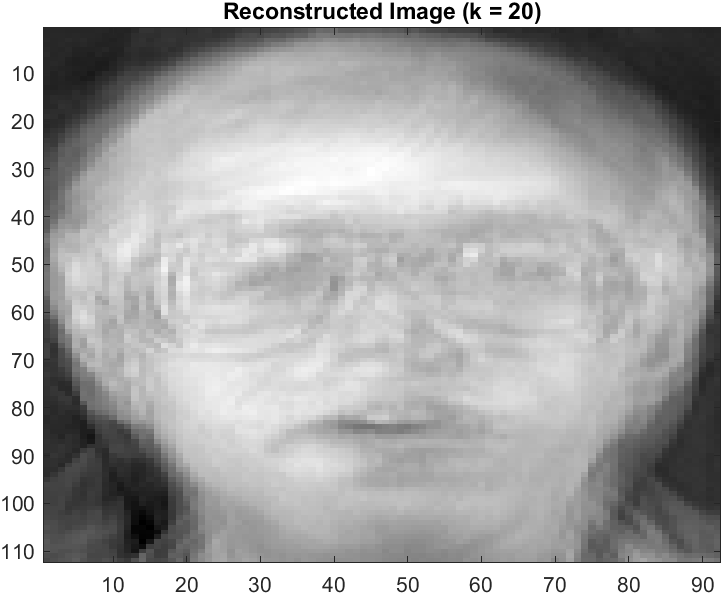
\includegraphics[width=\textwidth]{orl_recon_20.png}
        % \caption{Noisy \texttt{barbara256}}
    \end{minipage}
\end{figure}

\begin{figure}[!htb]
    \centering
    \begin{minipage}[b]{0.3\textwidth}
        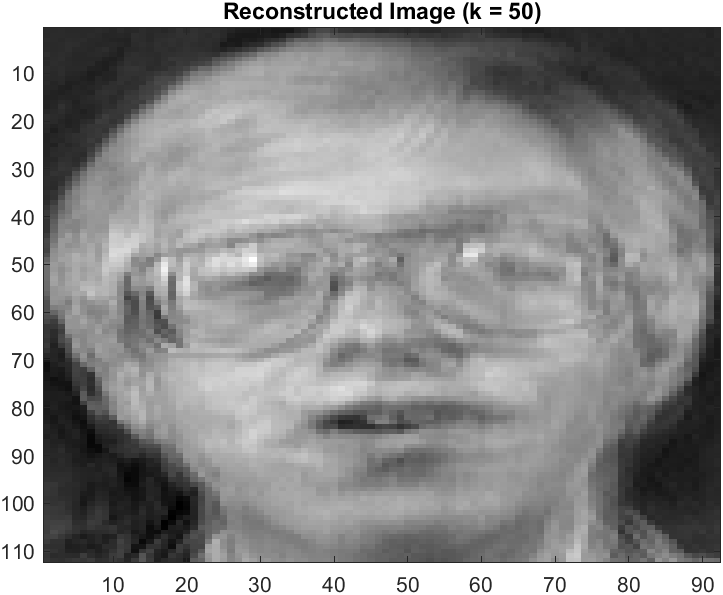
\includegraphics[width=\textwidth]{orl_recon_50.png}
        % \caption{Noisy \texttt{kodak24}}
    \end{minipage}
    % \hfill
    \begin{minipage}[b]{0.3\textwidth}
        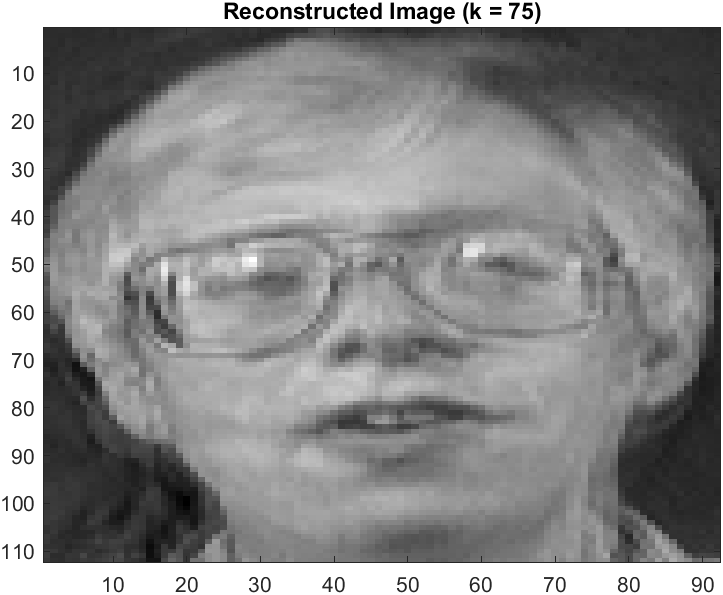
\includegraphics[width=\textwidth]{orl_recon_75.png}
        % \caption{Noisy \texttt{barbara256}}
    \end{minipage}
    % \hfill
    \begin{minipage}[b]{0.3\textwidth}
        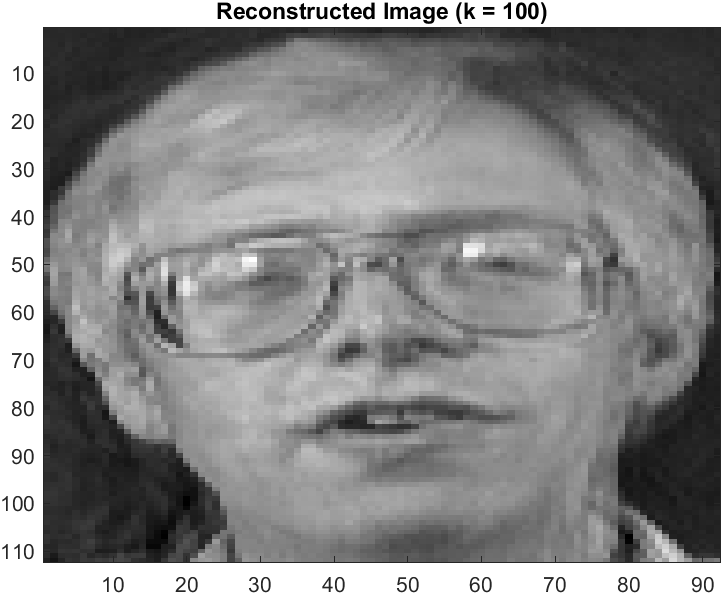
\includegraphics[width=\textwidth]{orl_recon_100.png}
        % \caption{Noisy \texttt{kodak24}}
    \end{minipage}
\end{figure}

\begin{figure}[!htb]
    \centering
    \begin{minipage}[b]{0.3\textwidth}
        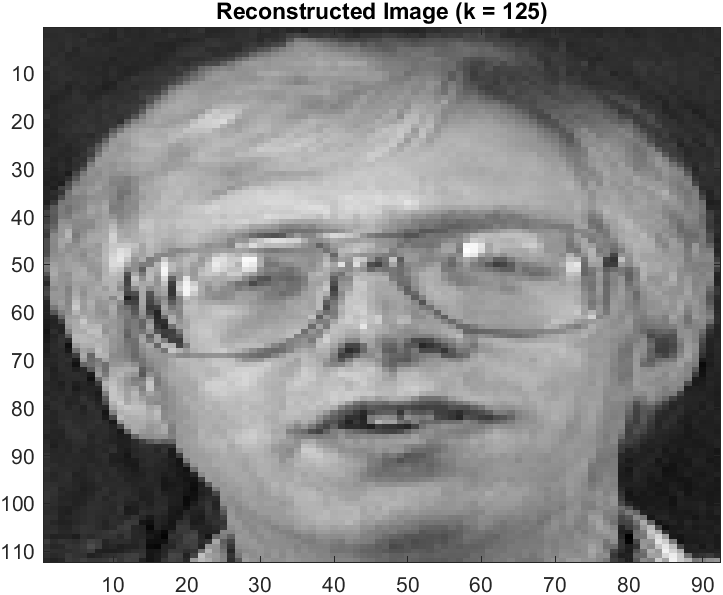
\includegraphics[width=\textwidth]{orl_recon_125.png}
        % \caption{Noisy \texttt{barbara256}}
    \end{minipage}
    % \hfill
    \begin{minipage}[b]{0.3\textwidth}
        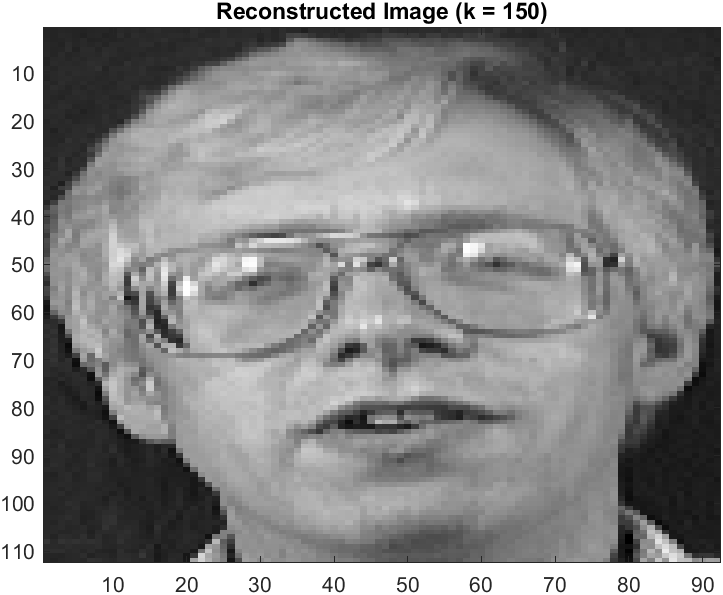
\includegraphics[width=\textwidth]{orl_recon_150.png}
        % \caption{Noisy \texttt{kodak24}}
    \end{minipage}
    % \hfill
    \begin{minipage}[b]{0.3\textwidth}
        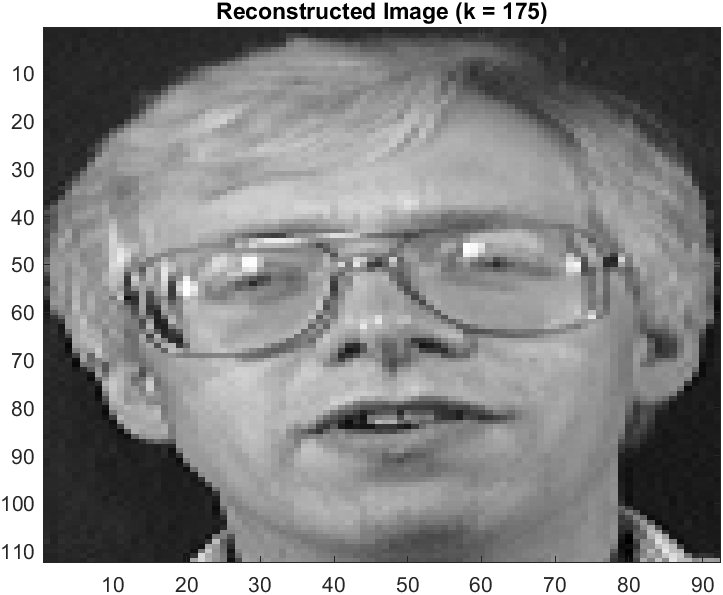
\includegraphics[width=\textwidth]{orl_recon_175.png}
        % \caption{Noisy \texttt{barbara256}}
    \end{minipage}
    % \hfill
\end{figure}

\newpage
The plot for 25 eigenvectors corresponding to the 25 largest eigenvalues is as follows:

\begin{figure}[!htb]
    \centering
    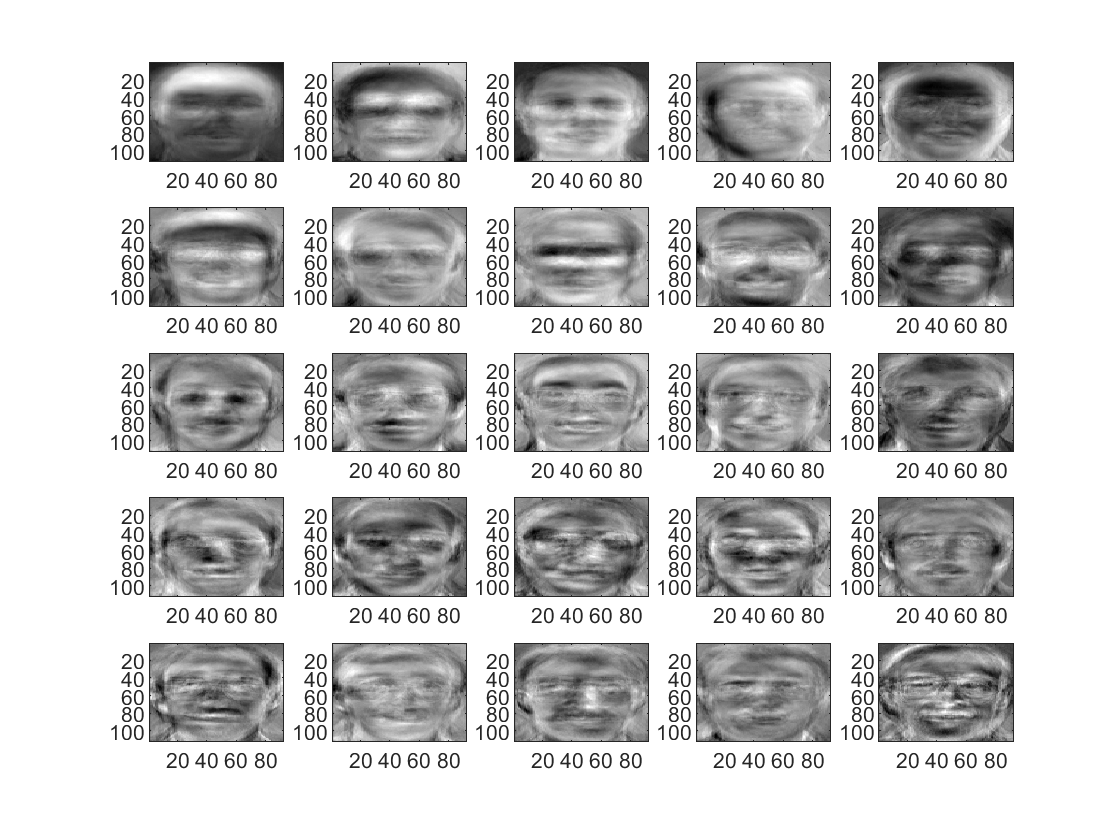
\includegraphics[width=\textwidth]{orl_25_subplot.png}
    % \caption{Recognition Rate using all the eigencoefficients for Yale dataset}
\end{figure}

\end{document}